\documentclass[10pt,a4paper]{scrartcl}
\PassOptionsToPackage{table}{xcolor}
\usepackage[utf8]{inputenc}
\usepackage[T1]{fontenc}
\usepackage[ngerman]{babel}
\usepackage{microtype, multicol, marginnote, bera, parskip}
\usepackage{listings, amsmath, amssymb, graphicx, tikz, epic}
\usepackage{stmaryrd} %for lightning arrow
\usepackage{pstricks, pst-node, pst-tree, pdflscape}
\usepackage[babel=true]{csquotes}
\usepackage{placeins}
\usepackage[labelformat=empty]{caption}
\tolerance=2000
\setcounter{secnumdepth}{0}
\usepackage[inner=2cm,outer=2cm,top=1.5cm,bottom=1.5cm,includeheadfoot]{geometry}
\usepackage{multirow}
\usepackage{float}
\newcommand{\subExercise}[1]{\vspace{0.5em} \noindent{\bf #1)}}
\newcommand{\B}{\mathbb{B}}
\DeclareMathOperator{\op}{op}

\author{Michael Mardaus \and Andrey Tyukin}
\title{
\includegraphics[scale=0.2]{../logo_schriftzug}\\
Technische Informatik: Abgabe 11}

\begin{document}

\maketitle

\section*{Exercise 11.1 (Johnny Simulator)}
\subExercise{a}
Program Listing:\\
\begin{tabular}{l|l|l}
Adr & Asm  & Op\\\hline
000 &  TAKE & 020\\
001 &  SUB  & 021\\
002 &  SAVE & 020\\
003 &  INC  & 022\\
004 &  TST  & 020\\
005 &  JMP  & 001\\
006 &  HLT  & 000\\
\end{tabular}

Puts $c = \lceil \frac{a}{b} \rceil$ (Adr 20 divided by Adr 21) into Adr 22.\\

\subExercise{b}
It takes $c$ times my loop (5 commands/cycles) plus 2 (TAKE and HLT) cycles.

\section*{Exercise 11.2 (Johnny Macro)}
The DBL macro would be a TAKE adr, ADD adr, SAVE adr combo.\\
The CLR macro would be a NULL adr, TAKE adr combo.

\section*{Exercise 11.3 (\emph{almost} Caesar-cipher)}
Our goal was to write an assembler program that performs the 
following computation:
\begin{verbatim}
// C or Java
for (i = 0; i < 10; i++) {
  a[i] = b[i] + c
}
\end{verbatim}
for some input array $b$, constant $c$ and output array $a$. 
Since we had no access to commercial operating systems, 
and also could not compile \textbf{Johnny} from source (no trace of any build-scripts or SCM?) \footnote{``Originally this code has not been designed to be published in an Open Source
Project. It probably contains a lot of passages that are hard to understand and
the code does certainly not fulfill the requirements of thorough
software engineering.
Some identifiers and comments are expressed German. Sorry for this ;-).'' - from "guido-main.pas" , \textbf{Johnny} source code. We absolutely empathise with the author of \textbf{Johnny}, but we too don't have any capacities to port it to Linux.}, we decided to implement it in NASM-assembler for x86 architectures, and to test it with well established emulators \textbf{Bochs} and \textbf{qemu-system-i386}. The result of the assembly is a stand-alone program, which can be executed without an operating system (it's actually a valid bootloader).

Here is the full listing:
\begin{verbatim}

; Tech Inf 2014 Exercise 11.3
;
; This program iterates through an array with 10 values,
; adds a constant to each value, 
; and saves the result in another array.
; 
; This program is supposed to be run directly on a computer with a
; x86 processor architecture, it does not require any operating system. 
; This is possible, because the resulting file assembled from this code 
; is a valid bootsector, which can be loaded directly by the BIOS.
;
; We use BIOS interrupts to output a message resulting from the addition 
; of the constant to the array: the resulting message should be "HelloWorld".
; The original array contains character codes of "HelloWorld" shifted by the
; constant. In this sense, this program demonstrates the usage of a very
; simple Caesar-cipher.
; After the message is printed, the program should hang until the computer
; is switched off.

[org 0x7c00] ; this is the address where our boot sector is loaded by BIOS

; just for the compliance with the question statement, here is the required offset
times 39 db 0 ; fill first 39 bytes with zeroes, start input array at 40th byte.

; this is the content of the original array, it's scrambled
encryptedString:
  db 'EbiilTloia'

; to make it reallyfunny, we write the result into the bootsector! xD
; here is some space for the result:
result:
  times 10 db 0

; the number '3' is the offset we used to produce the scrambled string above.
constant:
  db 3 

; we use bx as our pointer to the original array
mov bx, encryptedString

; load the constant into the register c
mov cl, [constant]

; now we loop through the array
addLoop:
  mov dl, [bx] ; move the number from array to register dl
  add dl, cl ; add the number with the constant
  add bx, 10 ; shift pointer forward
  mov [bx], dl ; write result
  sub bx, 9 ; shift pointer backward, increment by one
  cmp word bx, result ; check whether bx has reached the position 50
  je addEnd ; jump out of the loop if this is the case
  jmp addLoop ; otherwise continue looping through the array

addEnd:

; now we print the resulting array (i.e. string)
mov ah, 0x0e ; code of the BIOS interrupt for printing characters
mov bx, result ; move bx to the start of the result
printLoop:
  cmp word bx, constant ; check whether end of the array is reached
  je printEnd ; jump out of the loop if end of the array is reached
  mov al, [bx] ; load the character into the register
  int 0x10  ; call the interrupt to print the character
  add bx, 1 ; move to next character
  jmp printLoop ; keep printing

printEnd:
  jmp $ ; eternal loop, so that one can see the result.


times 510-($-$$) db 0  ; pad the boot sector to 512 bytes
dw 0xaa55 ; magic number for boot sectors, so that we can run it directly without OS
\end{verbatim}

The binary can be generated by running \textbf{make} (little bash-script in the folder with the source).
The emulators can be started by one of the following commands:
\begin{align*}
>&\textrm{bochs} \\
>&\textrm{qemu-system-i386 arrays.bin}
\end{align*}

The result looks as follows:
\begin{figure}[H]
  \centering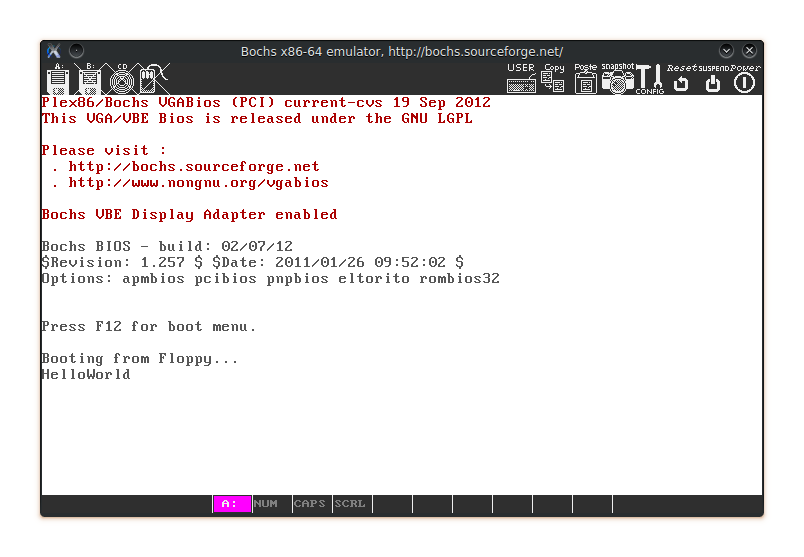
\includegraphics[width=0.9\linewidth]{images/helloWorld.png}
  \caption{Output of Bochs. The last line is the modified content of the array (as expected, decrypted to HelloWorld). Colors inverted to save some black ink.}
\end{figure}

\section*{Exercise 11.4 (Caches)}
\subExercise{a}
In a RAM with 32 addresses and a cache with 5 lines address 13 could be in cache line 3 in a direct mapped cache. And in any of the 5 cachelines in a fullassociative cache, depending on the used cache mapping algorithm.\\
\subExercise{b}
5 cache lines is an unusual amount for a 32 adress RAM because 32 cannot be distributed evenly.
Powers of 2 are common cache sizes. But the number of cachelines should at least divide the number of addresses.

\end{document}

